\documentclass[12pt]{article}
\usepackage{amsmath}
\usepackage{amsfonts}
\usepackage{fancyhdr}
\usepackage{titlesec}
\usepackage[margin=1in]{geometry}
\usepackage{siunitx}
\usepackage{booktabs}
\usepackage{graphicx}
\usepackage{float}
\usepackage[hidelinks]{hyperref}
\usepackage{todonotes}
\usepackage{rotating} % for rotating figures

\pagestyle{fancy}
\lhead{} 
\chead{} 
\rhead{\thepage} 
\lfoot{} 
\cfoot{} 
\rfoot{} 
\renewcommand{\headrulewidth}{0pt} 
\renewcommand{\footrulewidth}{0pt} 
%\titleformat{\section}[block]{\Large\bfseries\filcenter}{}{1em}{}
%\titleformat{\subsection}[block]{\large\bfseries\filcenter}{}{1em}{}
%To make sure we actually have header 0.5in away from top edge
%12pt is one-sixth of an inch. Subtract this from 0.5in to get headsep value
\setlength\headsep{0.333in}
\pagestyle{fancy}
\linespread{1.4}

\newcommand{\boldrule}{\rule{\linewidth}{2pt}} % Draws a thick line

\newcommand{\overbar}[1]{\mkern 1.5mu\overline{\mkern-1.5mu#1\mkern-1.5mu}\mkern 1.5mu} % Reduces length of \overline


\graphicspath{{Graphics/}}

\begin{document}

\thispagestyle{empty}
\newpage
\vspace*{3cm}
\begin{center}
%Lab title goes here
{\Huge EE 648 -- VLSI Design\\[.5cm]
Binary Coded Hexadecimal to Seven-Segment Display Converter}
\end{center}
\vspace{5mm}
\boldrule\\
\begin{center}

\includegraphics{uaflogo.png}\\[.5cm]
\boldrule\\[3cm]
{\Large
\textsc{Ryker Dial}\\
\textsc{Cody Gossel}\\
\textsc{Zach Krehlik}\\[1cm]
April 18, 2017
}
\end{center}


\newpage

\thispagestyle{empty}
\tableofcontents

\newpage

\setcounter{page}{1}

%Rest of report goes here

\section{Introduction}
The objective of this project is to design and fabricate an integrated circuit that takes four input bits representing a hexadecimal number and displays that number on a seven-segment display.
Such a circuit will be useful for a microcontroller because it reduces the number of pins required to use the display from seven to four, freeing up GPIO pins for other tasks.

%The goal of this project is to design and fabricate a chip that will use 4 input bits to control a 7 segment display. 
%An integrated circuit such as this can be used to connect a 7 segment display to a microcontroller, reducing the number of output pins required to drive the display.
%Four output pins of the controller are used to input the number to the IC, which then uses open collector outputs to pull down the cathodes of the 7 segment display. 


\section{Top Level Design}
To facilitate the design of this circuit, the logic for each segment is separated into its own module.
This converter is being designed for an active-low seven-segment display, so the output of each module will be used to switch a FET that pulls the segment to ground when switched on, turning on the segment.
The top-level design for the converter circuit with these modules included is shown in Figure \ref{fig:TopLevelCkt}.

%The general strategy with the design is to separate the logic for each segment into its own module.
%The output of each module will be used to switch a FET that drives the corresponding segment on the seven segment display.
%The top level diagram is shown in Figure \ref{fig:TopLevelCkt}.

\begin{figure}[H]
	\centering
	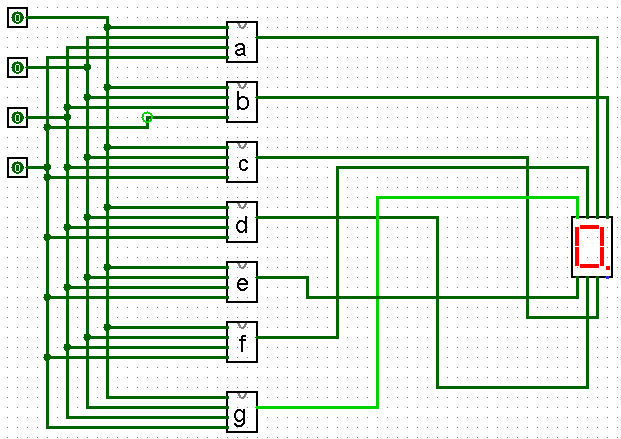
\includegraphics[width=\linewidth, keepaspectratio]{topLevelLogicCkt.png}
	\caption{Converter Top Level layout}
	\label{fig:TopLevelCkt}
\end{figure}

%Many of the gate level circuits use the inputs as well as their complements.  
%To reduce the number of gates in the final design, the inputs will each be inverted before being to the logic circuitry.  
%This will minimize redundancies in the gate layout.  
%This has not been included in this iteration of the design.


\section{Detailed Design}
\subsection{Gate Level} \label{sec:gateLevel}

The truth table for the converter, which includes its four inputs and seven outputs, is shown in Table \ref{tab:truthTable}.
A value of zero corresponds to the segment being on, and vice-versa.
From this, truth tables for each individual output were obtained and transferred to a program called Logisim, which is a free tool for designing and simulating logic circuits.
This tool was used to generate minimized NAND-only Boolean expressions for each module, as using only inverting logic will reduce the number of inverters required to realize the converter circuit.
Logisim was also used to generate the gate-level schematics for each module; the gate-level schematics for each module can be found in Appendix \ref{app:segmentLogic}, and the corresponding logic functions can be found in Appendix \ref{app:logicEquations}.

%The truth table for the four inputs and all seven outputs was created, it is shown in Figure \ref{fig:truthTable}.

\begin{table}[H]
	\centering
	\caption{Converter Truth Table}
	\vspace*{2mm}
	\label{tab:truthTable}
	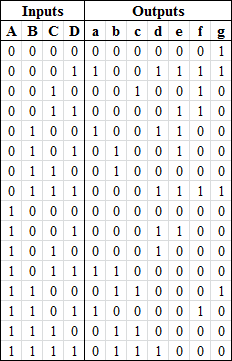
\includegraphics[width=0.4\linewidth, keepaspectratio]{hex7seg_truthTable.png}
\end{table}

\newpage
From the logic equations and gate-level schematics, note that the complement of any particular input is used many times.
In the actual implementation of the circuit, as opposed to what is shown in the gate-level schematics, the complements of the input signals will be produced only once and reused as needed, greatly reducing the number of inverters in the circuit.
Additionally, there are several terms in the logic equations that appear more than once: specifically $\overbar{(\bar{A}B\bar{C}\bar{D})}$, $\overbar{(AB\bar{C}D)}$, $\overbar{(AB\bar{D})}$, and $\overbar{(\bar{B}\bar{C}D)}$; the outputs of these gates will be reused as well.

To verify the functionality of the circuit, Logisim was used to simulate the output for each of the sixteen possible inputs.
The input and output waveforms were then plotted and are shown in Figure \ref{fig:BCD_sim}.
Comparing the simulated output to the converter circuit's truth table verifies that the design is valid.

%The truth table was transferred to the free software Logisim one output at a time.  
%Logisim analyzed the truth table for each output bit and generated a minimized NAND Boolean expression.  
%Utilizing inverting logic will reduce the number of inverters required to realize the circuit.
%Note that a zero in the output represents an active segment.
%The equivalent set of logic equations is shown in Appendix \ref{app:logicEquations}.

%Each logic equation represents a block on the top level diagram, and has a corresponding series of gates. The gate level design of these blocks is included in Appendix \ref{app:segmentLogic}.

\begin{figure}[H]
	\centering
	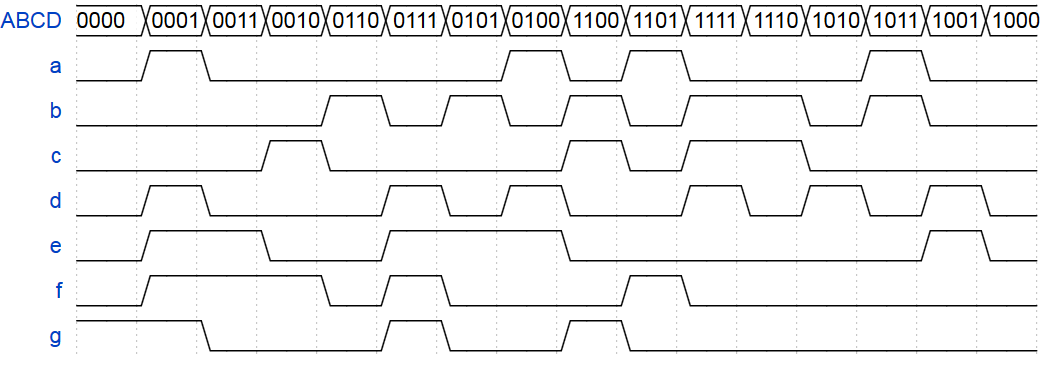
\includegraphics[width=\linewidth, keepaspectratio]{BCD_sim_waveform.png}
	\caption{Simulated Input and Output of Converter}
	\label{fig:BCD_sim}
\end{figure}

\subsection{Transistor Level}

\subsubsection{Transistor Level Schematics}

By using Logisim to implement each module with only NAND and inverter gates, the converter circuit can be realized with only a few gates: specifically two, three, and four input NAND gates, and an inverter.
Efficient implementations of these gates can be designed once and reused as needed, though different sizes of these gates will need to be made to optimize for delay and power consumption. 
The transistor level design of these gates is shown in Figures \ref{fig:2nandTran}, \ref{fig:3nandTran}, \ref{fig:4nandTran}, and \ref{fig:notTran}.
\begin{figure}[H]
	\centering
	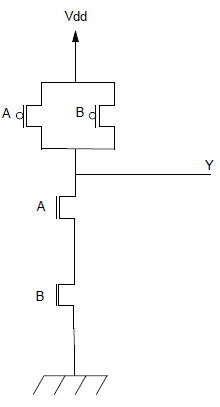
\includegraphics[width=0.3\linewidth, keepaspectratio]{NAND_2_Trans.png}
	\caption{Transistor Level Schematic for Two-Input NAND}
	\label{fig:2nandTran}
\end{figure}

\begin{figure}[H]
	\centering
	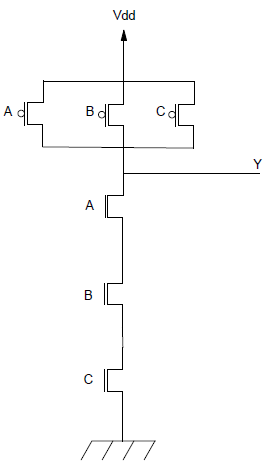
\includegraphics[width=0.3\linewidth, keepaspectratio]{NAND_3_Trans.png}
	\caption{Transistor Level Schematic for Three-Input NAND}
	\label{fig:3nandTran}
\end{figure}

\begin{figure}[H]
	\centering
	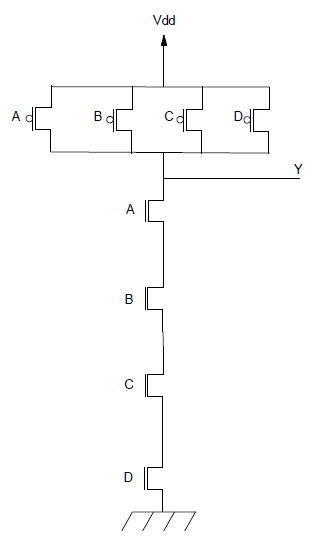
\includegraphics[width=0.3\linewidth, keepaspectratio]{NAND_4_Trans.png}
	\caption{Transistor Level Schematic for Four-Input NAND}
	\label{fig:4nandTran}
\end{figure}

\begin{figure}[H]
	\centering
	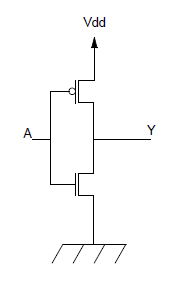
\includegraphics[width=0.3\linewidth, keepaspectratio]{NOT_Trans.png}
	\caption{Transistor Level Schematic for Inverter}
	\label{fig:notTran}
\end{figure}

\newpage
\subsubsection{Transistor/Gate Sizing}
Sizing the transistors to optimize for delay first requires knowing the input and output capacitance for each module of the converter circuit. 
In addition to the physical capacitance of the external connections to the circuit it is necessary to determine the capacitance of one normalized unit, generally referred to as \(C\).
Knowledge of these two values will allow for the application of the linear delay model.
The value of \(C\) is determined by constructing a unit inverter in Magic, and extracting it to a spice model.
A unit inverter has an input capacitance of \(3C\), and spice calculates the physical capacitance of the inverter to be \SI{221}{\femto\farad}.
Dividing this number by 3 yields the normalization factor of \SI{74}{\femto\farad}.

The input capacitance to the circuit is based off of an MSP430 output pin.
The capacitance of the output pin is readily availiable on a device datasheet, and is roughly \SI{5}{\pico\farad}.
This can be normalized to \(67C\) for the input to the circuit.

The output capacitance is based off of the open drain transistor which forms the output of the IC.
An example of an open drain circuit is shown in Figure \ref{fig:openCollector}.

\begin{figure}[H]
	\centering	
	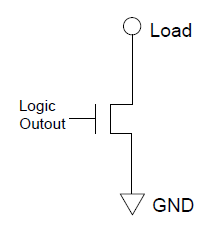
\includegraphics[width=0.4\linewidth, keepaspectratio]{openCollector.png}
	\caption{Block a Gate Level Schematic}
	\label{fig:openCollector}
\end{figure}

The nmos will present either a hi-z or low voltage to the external device.
One end of the external device is attached to an external voltage source, and the other is attached to the load pin of the nmos.
When the nmos is turned on it allows for current to flow through the LED, which causes it to light up. 

Sizing of the open drain transistor is determined by considering the current necessary for an LED segment and a desired voltage drop.
In order to keep dissipated power through the IC low, a \(Vds\) of 0.2 V is selected for the transistor.
The maximum current required will be approximately \SI{20}{\milli\ampere}.
These two values can be used with the long channel mosfet equations to determine a required channel width, assuming that the channel length will be held at the minimum.
The relation between transistor current and channel width is given by Equation \eqref{eq:chanCurrent}.

\begin{equation}
\label{eq:chanCurrent}
 I_{ds} = \mu C_{ox} \frac{W}{L} (V_{gt} - V_{ds}) V_{ds}
\end{equation}

There are several given values in the equation, \(\mu\), the electron mobility can be found in the spice technology file and is \SI{275}{\centi\meter\per\volt\squared}.
\(C_{ox}\) is the per area capacitance of the oxide layer, and is derived from the \SI{40}{\angstrom} oxide thickness used by TSMC.
\(V_{gt}\), \(V_{ds}\), and \(I_{ds}\) are based on the 3.3 V logic level of the IC less the threshold voltage of 0.7 V, the desired \(V_{ds}\) of 0.2 V, and the maximum expected current of 20 mA respectively.

Rearranging the equation and solving for \(W\) when \(L\) is fixed at \SI{180}{\nano\meter} results in a width of \SI{3.3e-5}{\meter}, which is approximately \(550 \lambda\) in magic.
The input capacitance of a transistor is proportional to the width, with each \(\lambda\) resulting in \(C\) worth of capacitance, so the open drain output is said to present \(550 C\) worth of capacitance to the logic circuit.

With values for the input and output capacitances is it possible to calculate the critical path delay for each module.
For modules a, b, d, and f the critical path is an un-inverted input feeding into a four-input NAND, the output of which is fed into another four-input NAND which produces the module output.
For modules c, e, and g the critical path is an un-inverted input feeding into a three-input NAND, the output of which is fed into another four-input NAND which produces the module output.
The delay for the worst case path can be found using the equation
\begin{equation}
	D = NF^{1/N}+P
\end{equation}
where \(N\) is the number of stages, \(F\) is the total path effort, and \(P\) is the combined parasitics of each gate in the path. F is calculated by the equation
\begin{equation}
	F = GBH
	\label{eqn:Path_Effort}
\end{equation}
where \(G\) is the path logical effort, \(B\) is the branching effort, and \(H\) is the path electrical effort, which is the output capacitance of the path divided by the input capacitance of the path.

\(G\) is the product of the individual logical efforts for each gate.
The logical effort for a three-input NAND is 5/3, and the logical effort for a four-input NAND is 6/3.
Thus, \(G\) for the critical path in modules a, b, d, and f is four, and the \(G\) for the critical path in modules c, e, and g is 10/3.
Since there is no branching in any of the circuits, the branching effort \(B\) for each path is one.
Each module has an input capacitance of 67C and an output capacitance of 550C, so \(H\) for each path is 8.2.
Using these values, the critical path effort for modules a, b, d, and f is 32.8 and the critical path effort for modules c, e, and g is 27.363.

With values for \(F\) it is possible to calculate the delay of the critical path for each circuit.
The parasitic for a three-input NAND is three and the parasitic for a four-input NAND is four, so the path parasitic for modules a, b, d, and f is eight, and the path parasitic for modules c, e, and g is seven. 
The number of stages in each critical path is two, so using Equation \ref{eqn:Path_Effort} the critical path delay for modules a, b, d, and f is 19.46 and the critical path for modules c, e, and g is 17.46.

To check whether these delays are close to optimal, the path effort \(F\) can be used to calculate the optimal number of stages, \(\hat{N}\) with the equation
\begin{equation}
	\hat{N} = log_4(F)
\end{equation}
For each module, the resulting optimal number of stages is three.
The three-stage critical path for each module is simply the two-stage critical path with an inverter placed at the input, and the calculated delays for these paths are 18.6 for modules a, b, d, and f and 17.0 for modules c, e, and g. 
Comparing these delays to the delays of the two-stage paths, the effect of adding another stage is so marginal that it is not worth it to add extra stages to the critical path, which would decrease the path effort and thus decrease the delay at the cost of higher power consumption.

Since the decrease in delay is not worth the increase in power, the critical paths remain unmodified in the circuit.
Thus, the gates in the critical paths can be sized using the equation
\begin{equation}
	C_{in} = \frac{C_{out}*g}{F^{1/N}}
\end{equation}
where \(C_{in}\) and \(C_{out}\) are the input and output capacitance of the gate and \(g\) is the logical effort of the gate.
Starting at the last gate, the output capacitance of the path is used to calculate the input capacitance, which determines the size of the gate; these calculations cascade until the end of the path is reached.
For the critical path for modules a, b, d, and f, stage one ends up having an input capacitance of 67C and stage 2 ends up having an input capacitance of 192C. 
By dividing these by the input capacitances of the corresponding unit-sized gates, this results in stage one having a size of 11 and stage two having a size of 32.
Similarly, stage one for modules c, e, and g has an input capacitance of 67C and a size of 11, and stage two has an input capacitance of 175C and a size of 29.
Since stage one for each critical path is a four-input NAND of size 11, only one four-input NAND gate will have to be designed for this stage.
The results of this section are summarized in Table \ref{tab:delay_sizing}.

\begin{table}[H]
	\centering
	\caption{Critical Path Delay and Stage Sizes}
	\label{tab:delay_sizing}
	\begin{tabular}{cccc}
		\toprule
		Modules & Critical Path Delay & Stage One Size & Stage Two Size	\\
		\midrule
		a,b,d,f & 19.5 & 11 & 32\\
		c,e,g & 17.5 & 11 & 29\\
		\bottomrule
	\end{tabular}
\end{table}

\section{Magic VLSI Layout}
\subsection{Individual Gate Layout}
Implementing the circuit in bare silicon required first constructing VLSI layouts for each gate.
To ease the assemblage of the full layout, the layout was started by designing every gate to be unit sized; this allows for expedient construction of the circuit and verification of the layout.
Additionally, the gates were laid out such that increasing the transistor size increases the width of the layout, while the height stays constant.
The \(V_{dd}\) and \(gnd\) rails of the transistor are at the top and bottom of the layout, respectively, so this means that resizing the transistors does not move the voltage rails.
These design choices make it easier to size the gates for optimal delay at a later date.

Figures \ref{fig:magic_inv}, \ref{fig:magic_NAND2}, \ref{fig:magic_NAND3}, and \ref{fig:magic_NAND4} in Appendix \ref{app:magic_vlsi_layouts} show the VLSI layouts for the inverter and the two, three, and four input NAND gates.
The functionality of each gate was verified by simulation with ngspice.
Figures \ref{fig:spice_INV}, \ref{fig:spice_2NAND}, \ref{fig:spice_3NAND}, and \ref{fig:spice_4NAND} in Appendix \ref{app:spice} show these simulations.

During simulations the delay, rise, and fall times were also measured from visual inspection of the waveform.
Delay is measured from 50\% on the input to 50\% on the output, the rise time is measured from 20\% on the output to 80\% on the output, and fall time is measured from 80\% on the output to 20\% on the output; Figure \ref{fig:delay_rise_fall} shows an example of how these were determined.
For the two, three, and four input NAND gates, the circuits used to test the delay, rise, and fall times consisted of the device under test, with a unit inverter on each input and the output driving four inputs to circuits of the same type.
Figure \ref{fig:nand_delay_meas} shows this setup for the 2-input NAND.

For the inverter circuit, the fan-out-of-four delay (FO4) was measured; the setup for this is shown in Figure \ref{fig:inv_delay_meas}.
Table \ref{tab:tran_dim} shows these measurements, as well as the physical dimensions of each gate.

\begin{table}[H]
	\centering
	\caption{Transistor Delay, Rise, and Fall Times}
	\label{tab:tran_dim}
	\begin{tabular}{lccccccc}
		\toprule
		Gate & Rise & Fall & \begin{tabular}{@{}c@{}}Falling \\ Delay \end{tabular} & \begin{tabular}{@{}c@{}}Rising \\ Delay \end{tabular} &  Width & Height & Area\\
		\midrule
		INV		& 50 ps & 55 ps & 40 ps & 40 ps &	128\(\lambda\) &	86\(\lambda\)	& 11,008\(\lambda^2\)	\\
		2NAND	& 135 ps & 120 ps &   120 ps &   90 ps  &	128\(\lambda\)	&	90\(\lambda\) 	& 11,520\(\lambda^2\)	\\
		3NAND	& 215 ps & 130 ps & 135 ps & 100 ps &	128\(\lambda\) &	94\(\lambda\) 	& 12,032\(\lambda^2\)	\\
		4NAND	& 265 ps & 155 ps & 185 ps & 110 ps &	128\(\lambda\)	&	98\(\lambda\) 	& 12,544\(\lambda^2\)	\\
		\bottomrule
	\end{tabular}
\end{table}

\subsection{Full Circuit Layout}
After constructing the individual gates, the next step was to lay them out into the full converter circuit.
To accomplish this, first each segment was laid out according to the logic diagrams in Appendix \ref{app:logicEquations}.
An example of the layout for an individual gate is shown in Figure \ref{fig:segA_layout} in Appendix \ref{app:magic_vlsi_layouts}.
The gates were laid out in a single line so that their \(V_{dd}\) and \(gnd\) rails would line up, starting with the gates in the first stage at the top and the gate in the last stage at the bottom.
Additionally, to the left of the \(V_{dd}\) rail there are rails for the A, B, C, and D inputs, and to the right of the \(gnd\) rail are rails for the inverted inputs needed by that segment.
Each segment includes inverters to generate the inverted inputs to reduce the inverter fan-out.
The inputs are only inverted once per segment, however, so some fan-out remains; fortunately the maximum fanout in this case is only three, which is acceptable for the purposes of this converter.

Each segment was laid out in this fashion, then all of the segments were combined into a full layout.
In Appendix \ref{app:magic_vlsi_layouts}, Figure \ref{fig:hex7seg_unexpanded} shows this layout with the individual cells unexpanded so that the location of each segment can be easily seen, and Figure \ref{fig:hex7seg_expanded} shows the layout with the individual cells expanded.
In this layout the segments are placed side-by-side, starting with segment a on the left and ending with segment g on the right.
At the top of the circuit are rails for \(V_{dd}\) and \(gnd\), and at the bottom are rails for the inputs A, B, C, and D.
This final layout has a width of 1769\(\lambda\) and a height of 947\(\lambda\).

\begin{figure}[H]
	\centering
	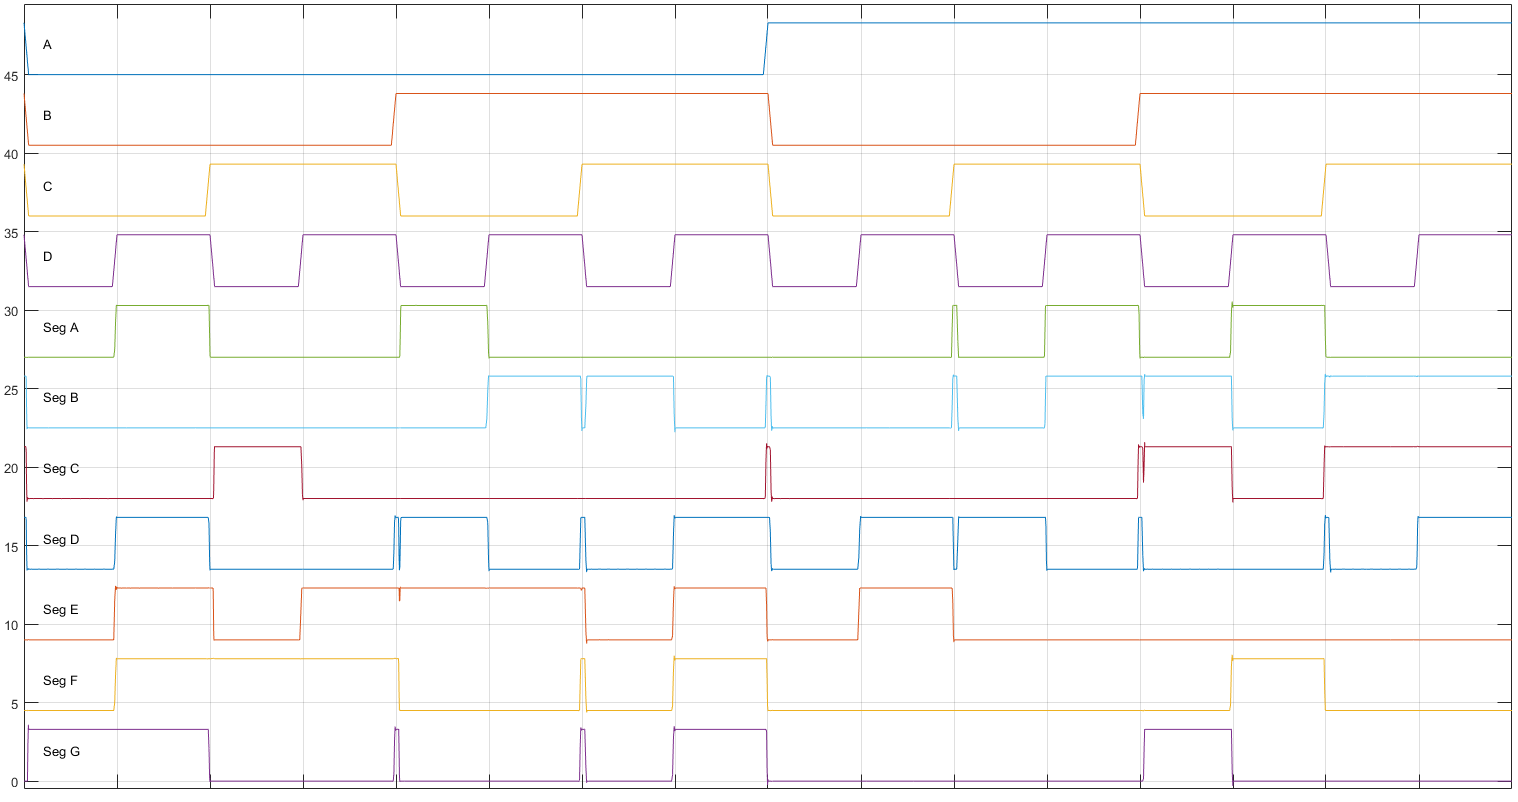
\includegraphics[width=\textwidth, keepaspectratio]{Graphics/7seg.png}
	\caption{Spice Simulation of Complete Circuit}
	\label{}
\end{figure}

\begin{figure}[H]
	\centering
	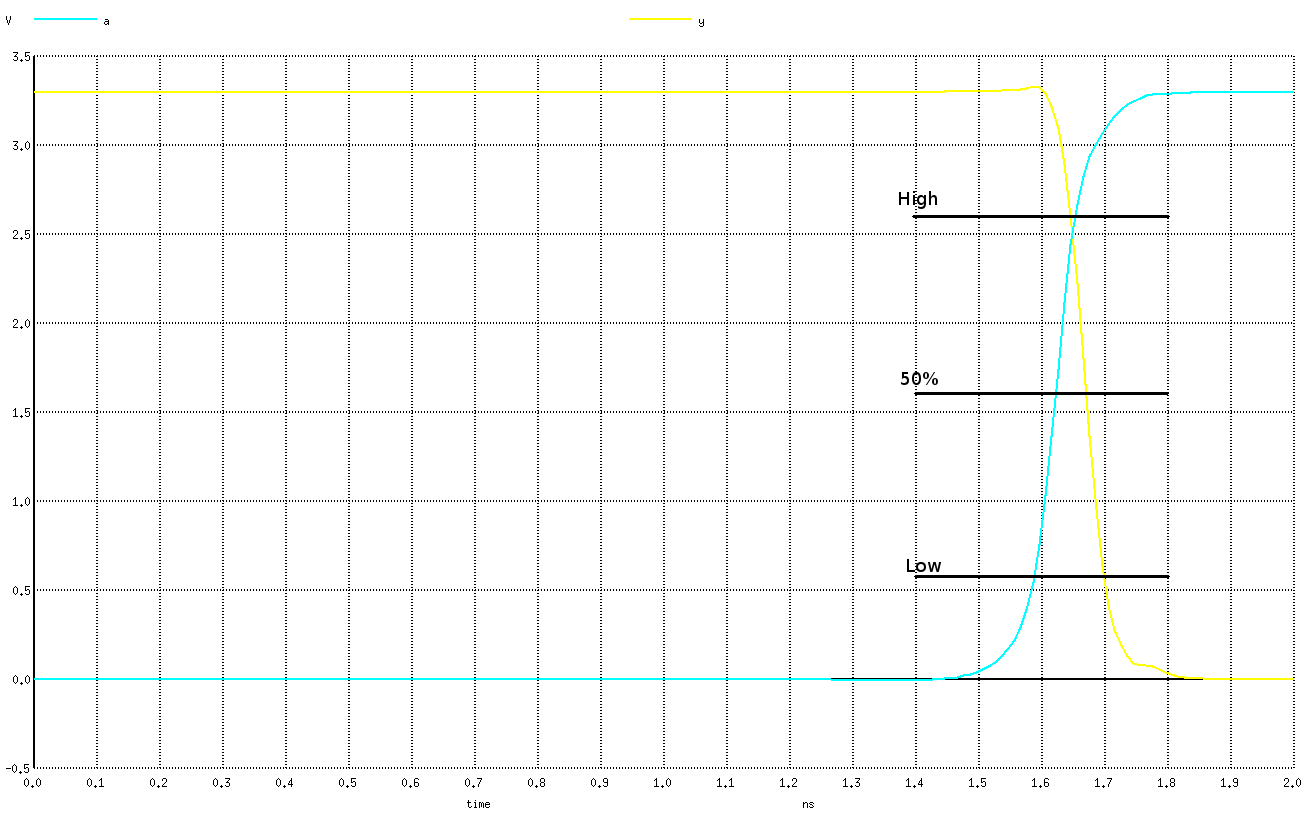
\includegraphics[width=\textwidth, keepaspectratio]{Graphics/FO4_Delay}
	\caption{Measuring FO4 Delay and Rise/Fall Times of Inverter}
	\label{fig:delay_rise_fall}
\end{figure}

\begin{figure}[H]
	\centering
	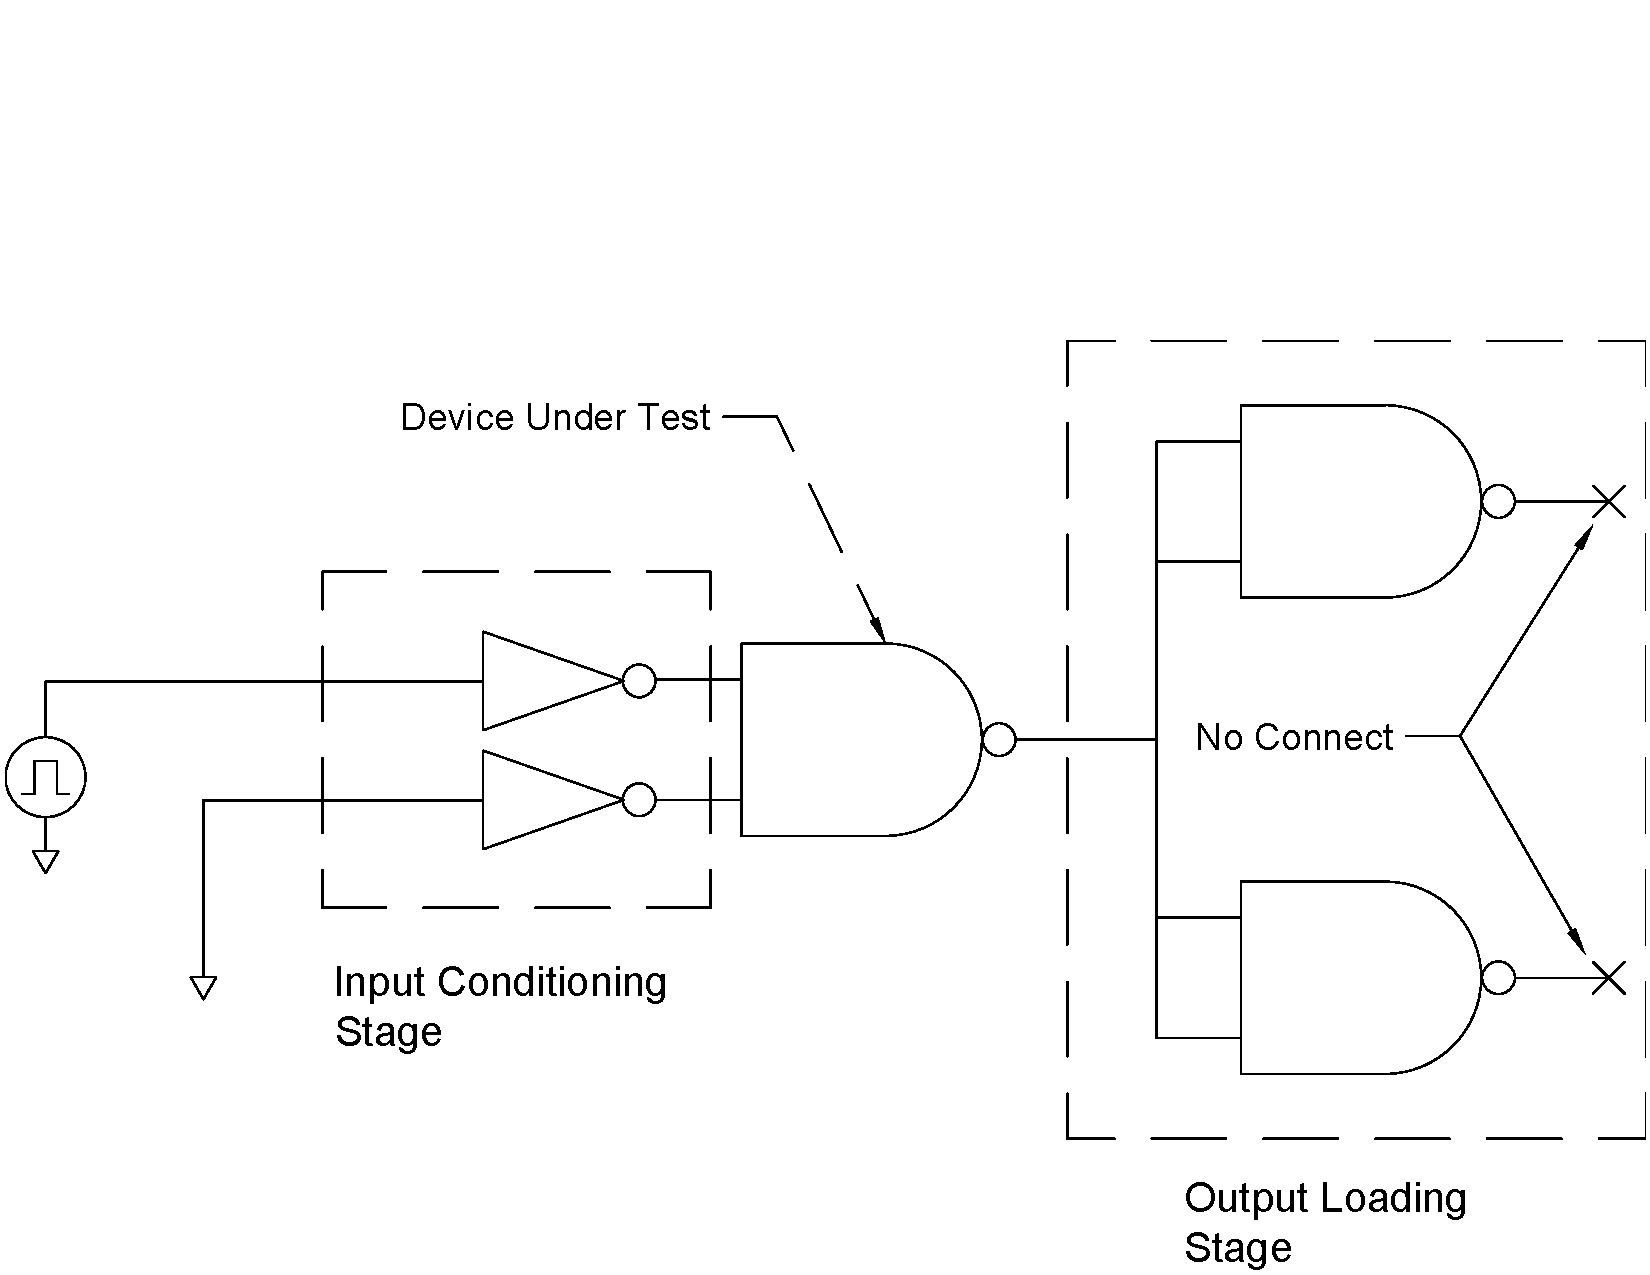
\includegraphics[width=\textwidth, keepaspectratio]{Graphics/NAND_FO4}
	\caption{Delay and Rise/Fall Time Measurement Setup for NAND Gates}
	\label{fig:nand_delay_meas}
\end{figure}

\begin{figure}[H]
	\centering
	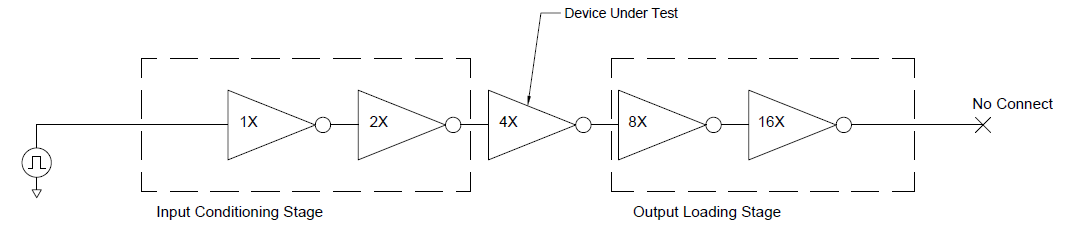
\includegraphics[width=\textwidth, keepaspectratio]{Graphics/INV_FO4}
	\caption{Delay and Rise/Fall Time Measurement Setup for Inverter}
	\label{fig:inv_delay_meas}
\end{figure}

\newpage
\appendix
\section{Segment Logic Diagrams}
\label{app:segmentLogic}
% Segment a ==============================================
\subsection{Segment a}

\begin{figure}[H]
	\centering
	\label{fig:aBlockGates}
	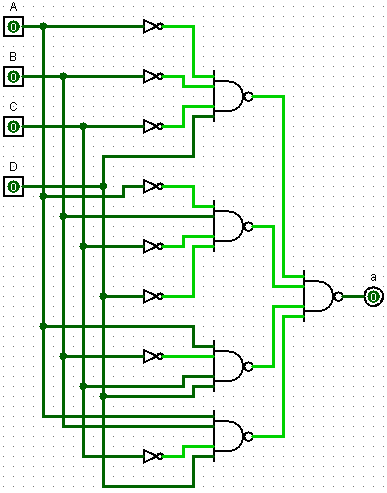
\includegraphics[width=0.5\linewidth, keepaspectratio]{a_logicCkt}
	\caption{Block a Gate Level Schematic}
\end{figure}

%Segment b ================================================
\subsection{Segment b}

\begin{figure}[H]
	\centering
	\label{fig:bBlockGates}
	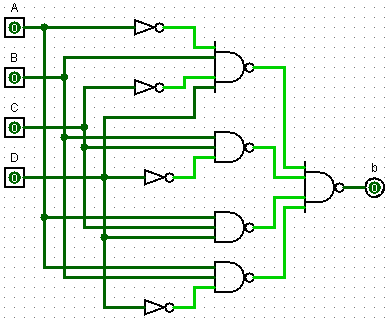
\includegraphics[width=0.5\linewidth, keepaspectratio]{b_logicCkt}
	\caption{Block b Gate Level Schematic}
\end{figure}

%Segment c ================================================
\subsection{Segment c}
\begin{figure}[H]
	\centering
	\label{fig:cBlockGates}
	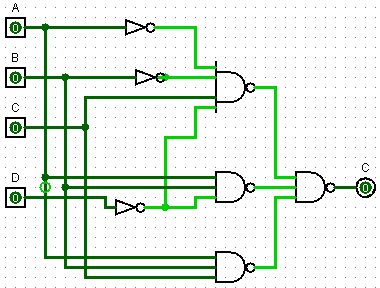
\includegraphics[width=0.5\linewidth, keepaspectratio]{c_logicCkt}
	\caption{Block c Gate Level Schematic}
\end{figure}

%Segment d =================================================
\subsection{Segment d}
\begin{figure}[H]
	\centering
	\label{fig:dBlockGates}
	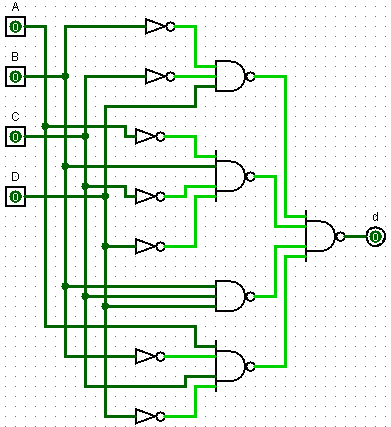
\includegraphics[width=0.65\linewidth, keepaspectratio]{d_logicCkt}
	\caption{Block d Gate Level Schematic}
\end{figure}

%Segment e ================================================
\subsection{Segment e}
\begin{figure}[H]
	\centering
	\label{fig:eBlockGates}
	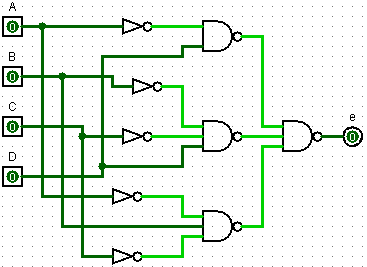
\includegraphics[width=0.65\linewidth, keepaspectratio]{e_logicCkt}
	\caption{Block e Gate Level Schematic}
\end{figure}

%Segment f ================================================
\subsection{Segment f}
\begin{figure}[H]
	\centering
	\label{fig:fBlockGates}
	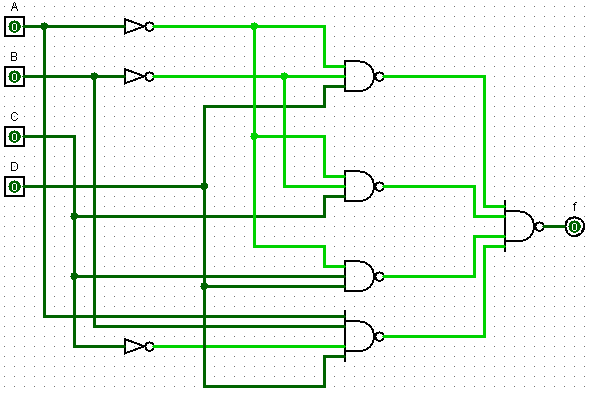
\includegraphics[width=0.65\linewidth, keepaspectratio]{f_logicCkt}
	\caption{Block f Gate Level Schematic}
\end{figure}

%Segment g ================================================
\subsection{Segment g}
\begin{figure}[H]
	\centering
	\label{fig:gBlockGates}
	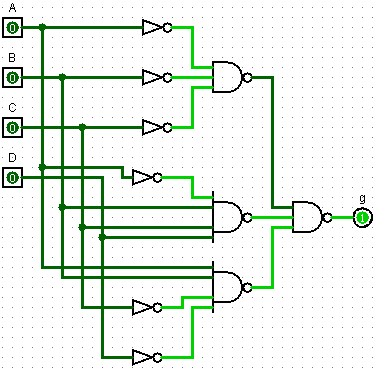
\includegraphics[width=0.65\linewidth, keepaspectratio]{g_logicCkt}
	\caption{Block g Gate Level Schematic}
\end{figure}


\newpage
\section{Logic Equations}
\label{app:logicEquations}
\begin{equation}
a = \overline{\overbar{(\bar{A}\bar{B}\bar{C}D)}\overbar{(\bar{A}B\bar{C}\bar{D})}\overbar{(A\bar{B}CD)}\overbar{(AB\bar{C}D)}}
\end{equation}

\begin{equation}
b = \overline{\overbar{(\bar{A}B\bar{C}D)}\overbar{(BC\bar{D})}\overbar{(ACD)}\overbar{(AB\bar{D})}}
\end{equation}

\begin{equation}
c = \overline{\overbar{(\bar{A}\bar{B}C\bar{D})}\overbar{(AB\bar{D})}\overbar{(ABC)}}
\end{equation}

\begin{equation}
d = \overline{\overbar{(\bar{B}\bar{C}D)}\overbar{(\bar{A}B\bar{C}\bar{D})}\overbar{(BCD)}\overbar{A\bar{B}C\bar{D}}}
\end{equation}

\begin{equation}
e = \overline{\overbar{(\bar{A}D)}\overbar{(\bar{B}\bar{C}D)}\overbar{(\bar{A}B\bar{C})}}
\end{equation}

\begin{equation}
f = \overline{\overbar{(\bar{A}\bar{B}D)}\overbar{(\bar{A}\bar{B}C)}\overbar{(\bar{A}CD)}\overbar{(AB\bar{C}D)}}
\end{equation}

\begin{equation}
g = \overline{\overbar{(\bar{A}\bar{B}\bar{C})}\overbar{(\bar{A}BCD)}\overbar{(AB\bar{C}\bar{D})}}
\end{equation}

\newpage
\section{Magic VLSI Layouts}
\label{app:magic_vlsi_layouts}

\begin{figure}[H]
	\centering
	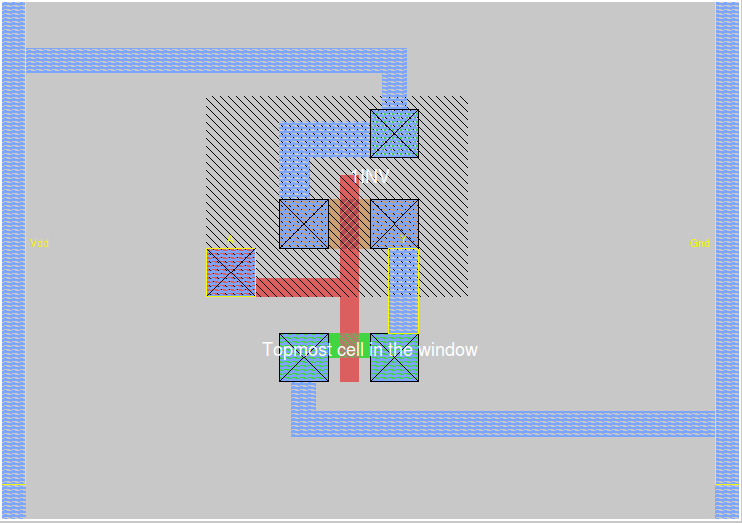
\includegraphics[width=0.70\linewidth, keepaspectratio]{Graphics/1INV}
	\caption{VLSI Layout for Inverter}
	\label{fig:magic_inv}
\end{figure}

\begin{figure}[H]
	\centering
	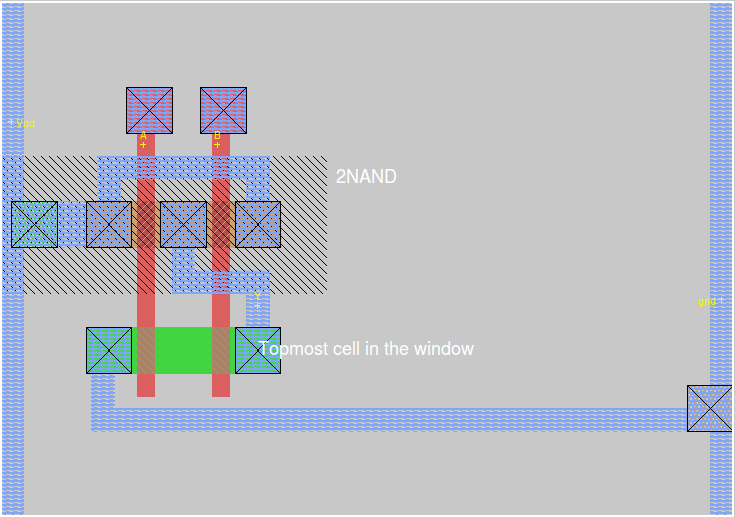
\includegraphics[width=0.70\linewidth, keepaspectratio]{Graphics/2NAND}
	\caption{VLSI Layout for 2-Input NAND}
	\label{fig:magic_NAND2}
\end{figure}

\begin{figure}[H]
	\centering
	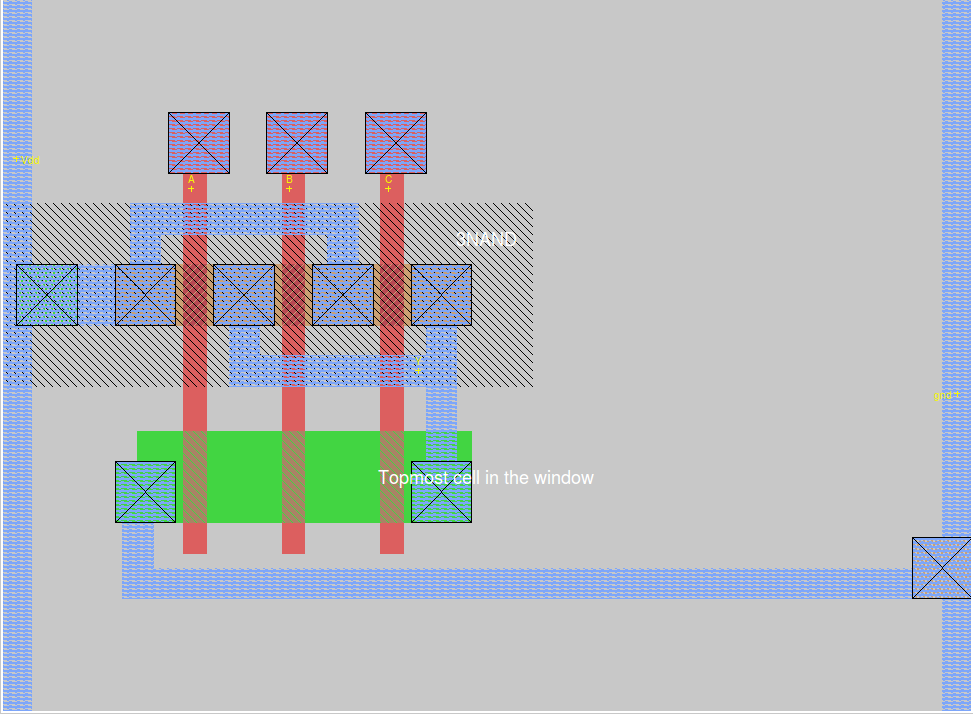
\includegraphics[width=0.70\linewidth, keepaspectratio]{Graphics/3NAND}
	\caption{VLSI Layout for 3-Input NAND}
	\label{fig:magic_NAND3}
\end{figure}

\begin{figure}[H]
	\centering
	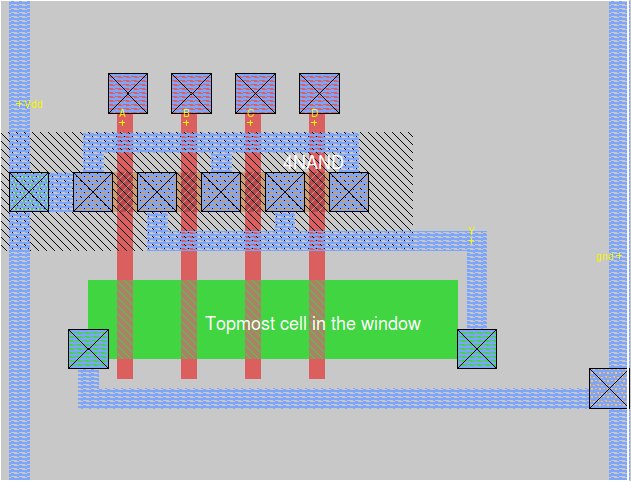
\includegraphics[width=0.70\linewidth, keepaspectratio]{Graphics/4NAND}
	\caption{VLSI Layout for 4-Input NAND}
	\label{fig:magic_NAND4}
\end{figure}

\begin{figure}[H]
	\centering
	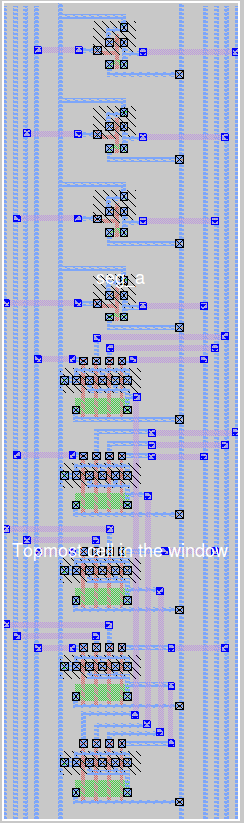
\includegraphics[width=0.42\linewidth]{Graphics/seg_a}
	\caption{Layout for Segment A}
	\label{fig:segA_layout}
\end{figure}
\clearpage
\begin{sidewaysfigure}
\centering
	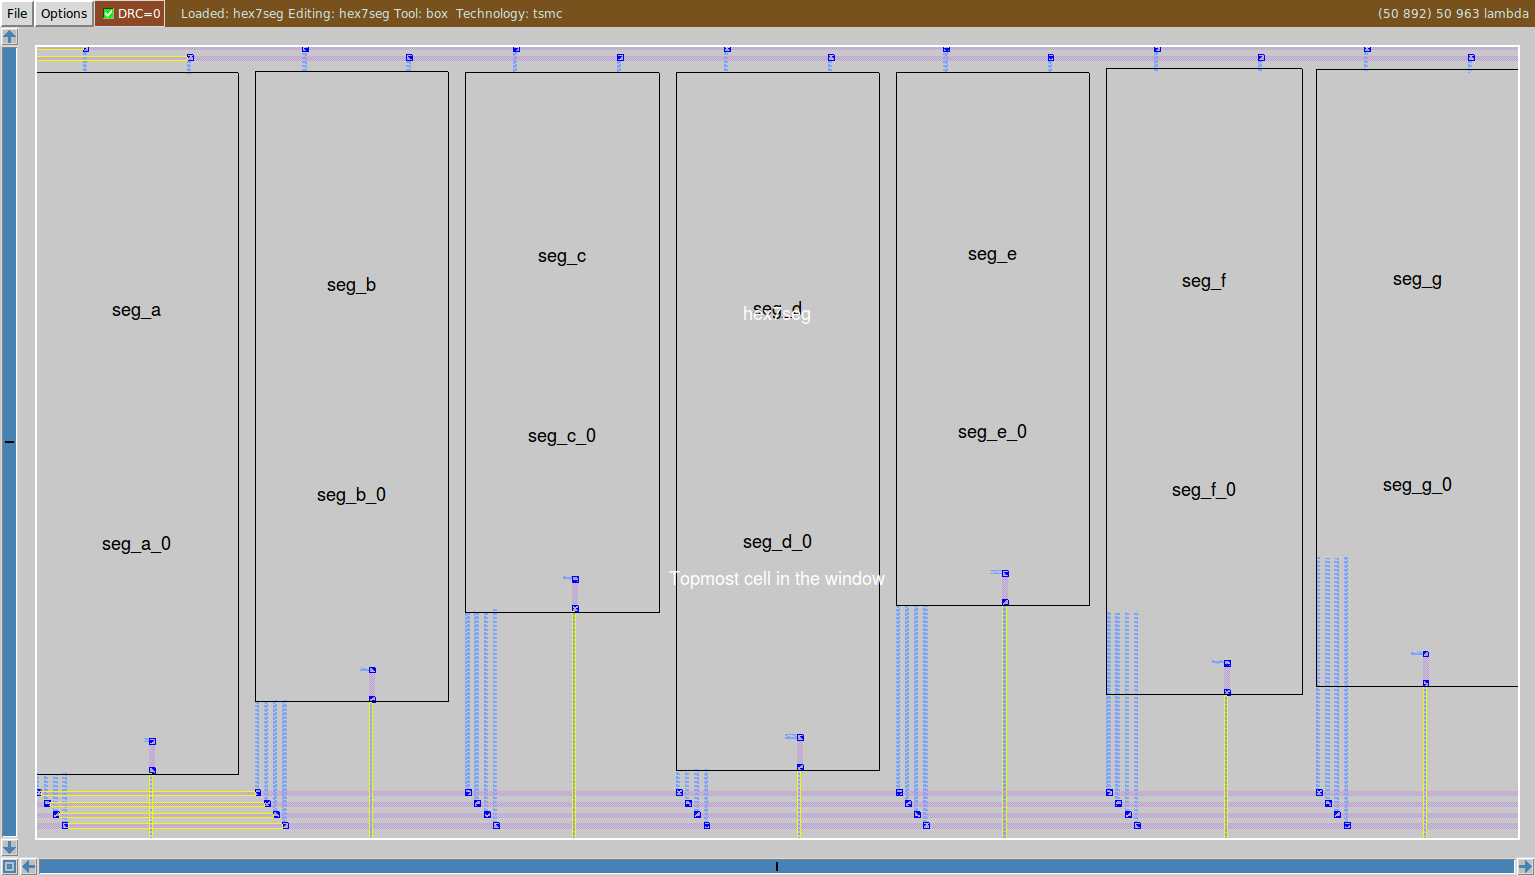
\includegraphics[width=\textwidth]{Graphics/hex7seg_unexpanded}
	\caption{Unexpanded Full Circuit Layout}
	\label{fig:hex7seg_unexpanded}
\end{sidewaysfigure}
\clearpage
\begin{sidewaysfigure}
	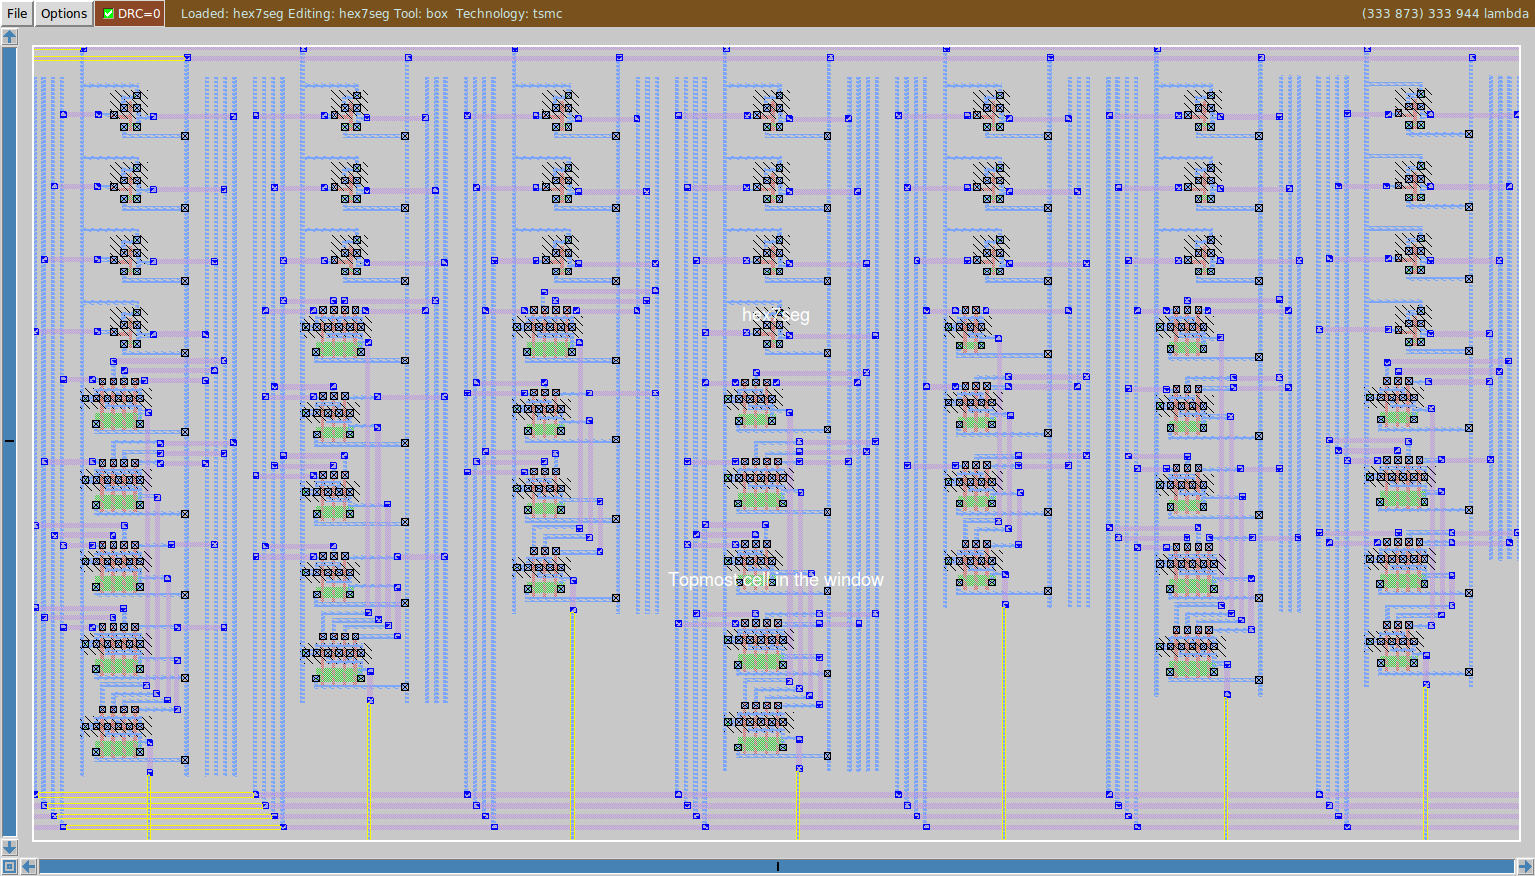
\includegraphics[width=\textwidth]{Graphics/hex7seg_expanded}
	\caption{Expanded Full Circuit Layout}
	\label{fig:hex7seg_expanded}
\end{sidewaysfigure}
\clearpage
\section{SPICE Simulations}
\label{app:spice}

\begin{figure}[H]
	\centering
	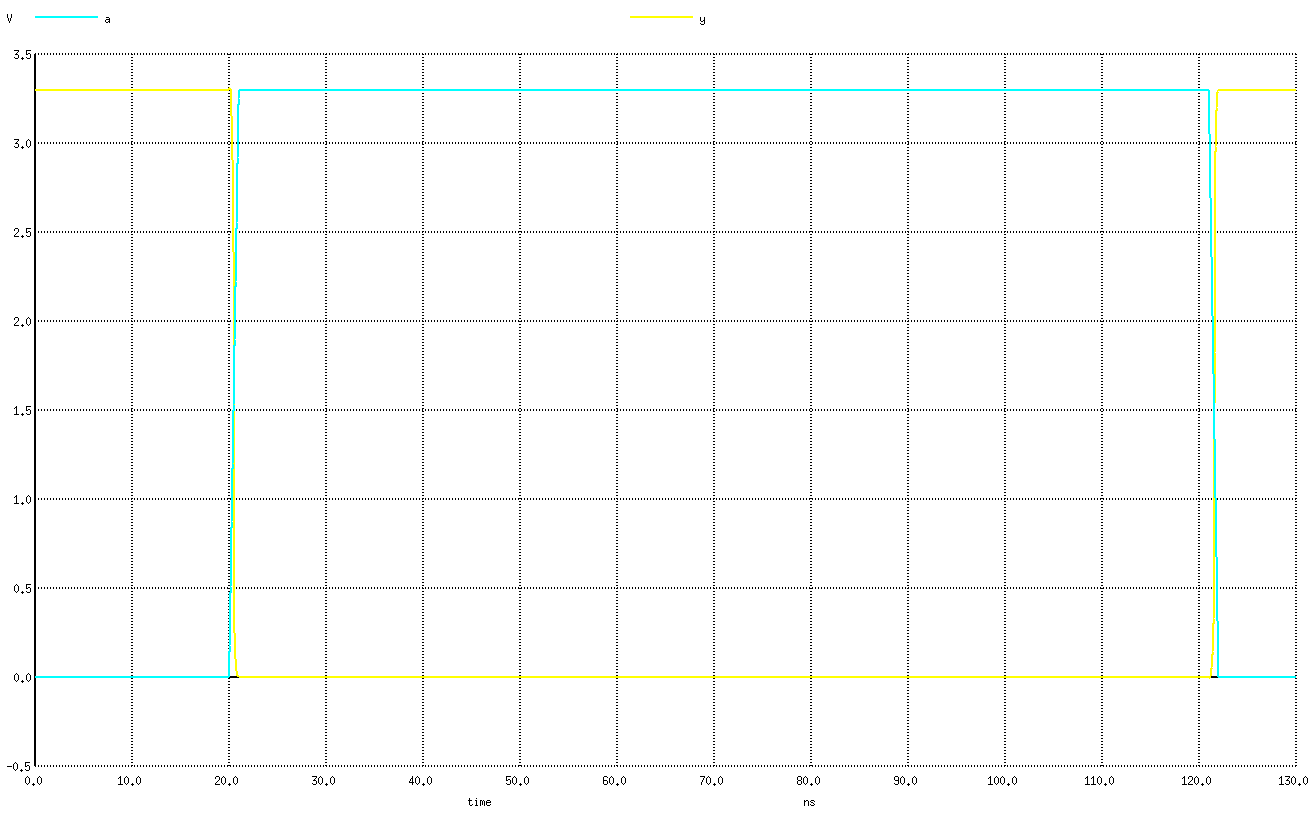
\includegraphics[width=0.70\linewidth, keepaspectratio]{Graphics/1INV_spice}
	\caption{Spice Simulation of Unit Inverter}
	\label{fig:spice_INV}
\end{figure}

\begin{figure}[H]
	\centering
	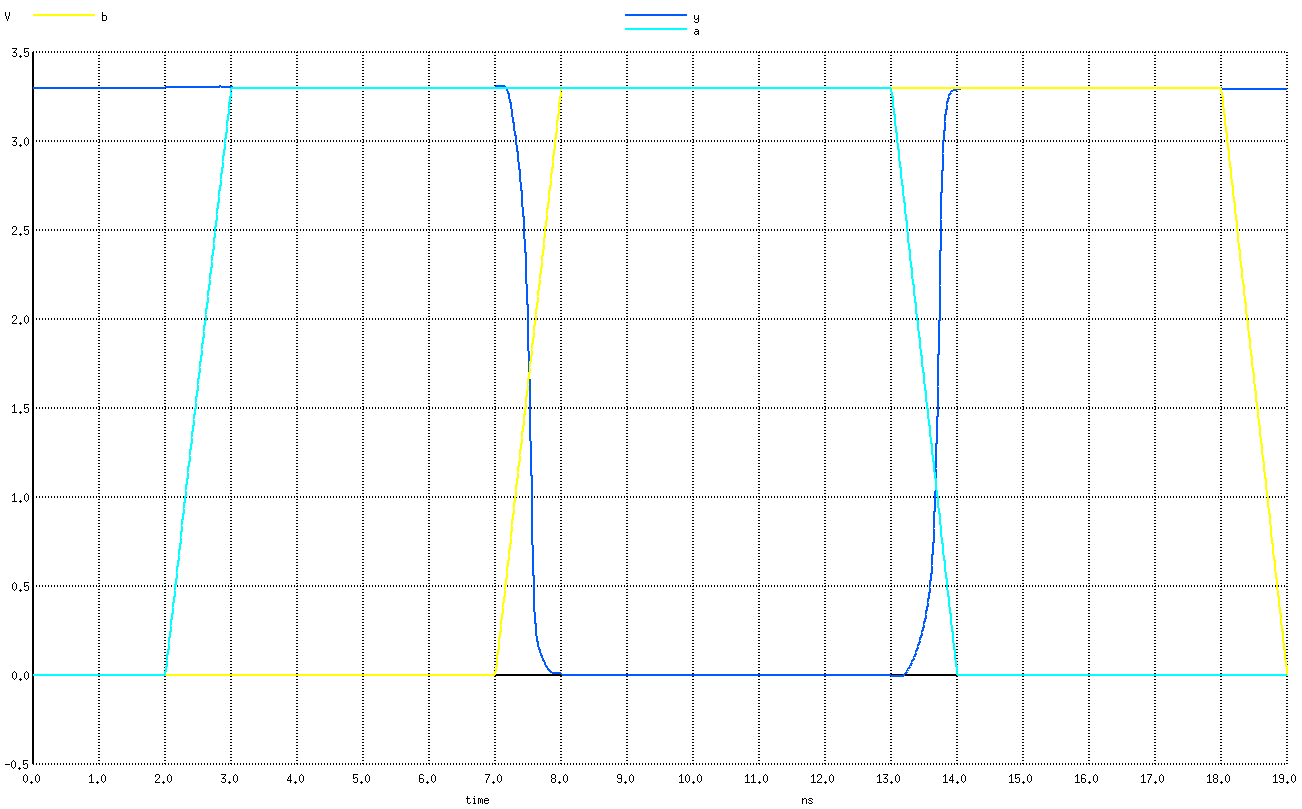
\includegraphics[width=0.70\linewidth, keepaspectratio]{Graphics/2NAND_spice}
	\caption{Spice Simulation of 2-Input NAND}
	\label{fig:spice_2NAND}
\end{figure}

\begin{figure}[H]:
	\centering
	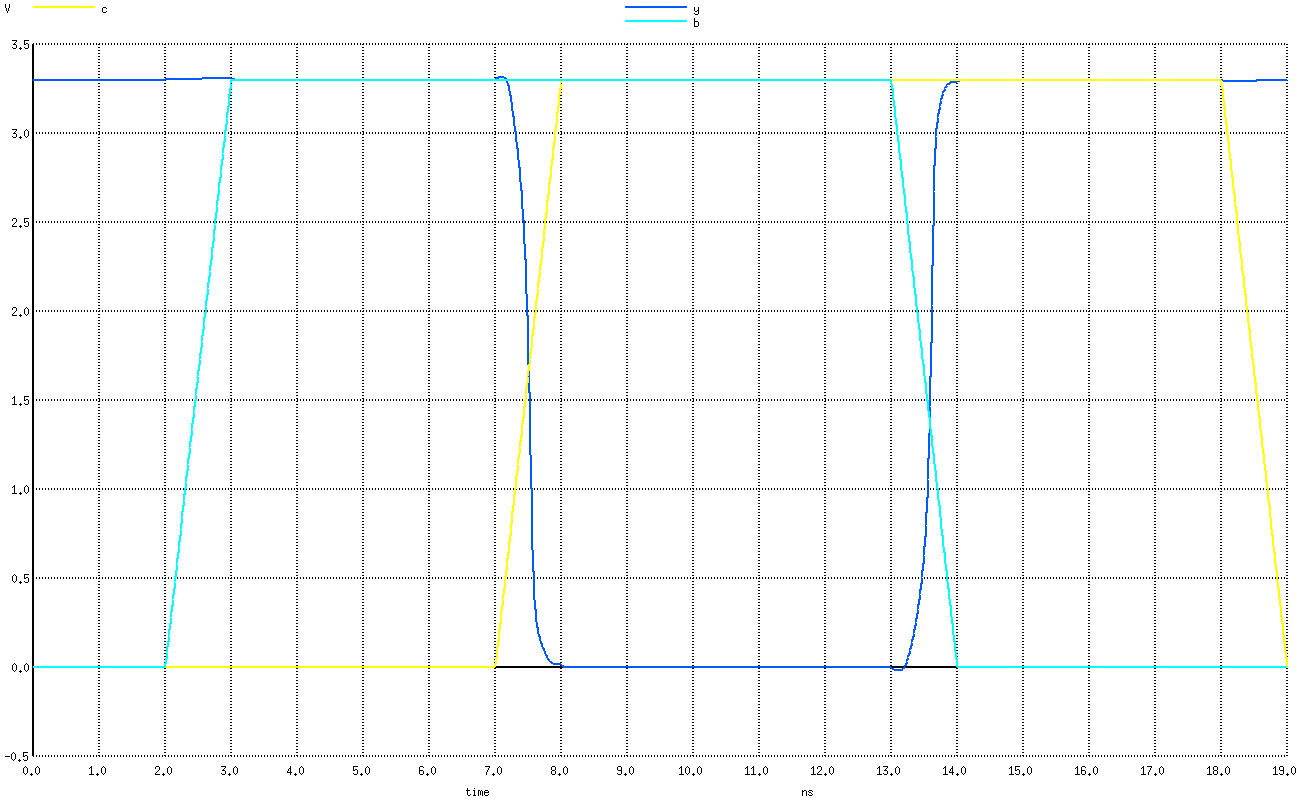
\includegraphics[width=0.70\linewidth, keepaspectratio]{Graphics/3NAND_spice}
	\caption{Spice Simulation of 3-Input NAND}
	\label{fig:spice_3NAND}
\end{figure}

\begin{figure}[H]
	\centering
	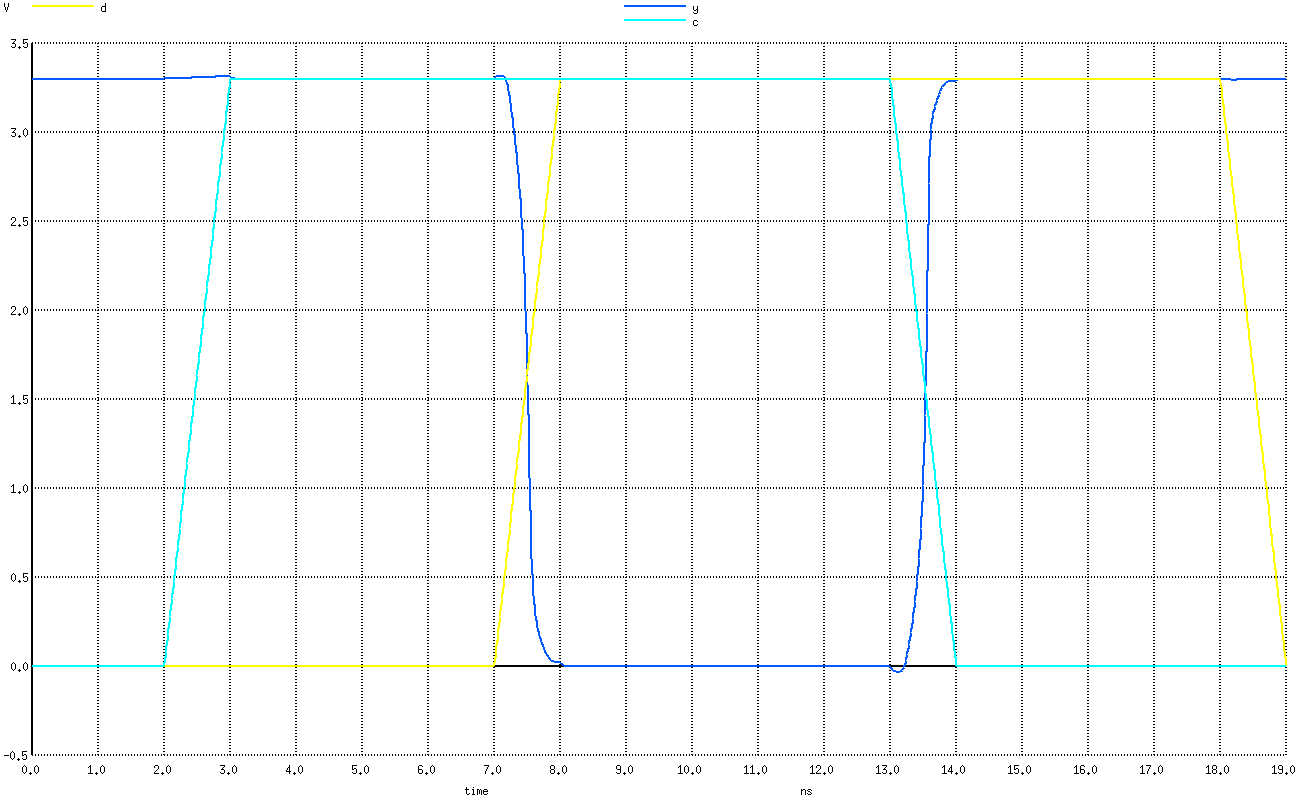
\includegraphics[width=0.70\linewidth, keepaspectratio]{Graphics/4NAND_spice}
	\caption{Spice Simulation of 4-Input NAND}
	\label{fig:spice_4NAND}
\end{figure}

\end{document}
